\chapter{Silnik}

Rozdział ten opisuje główny komponent tworzonego systemu nazwanego Silnikiem. Odpowiedzialny jest on za dostarczenie interfejsu definiowania trójwymiarowej wizualizacji i~jej późniejsze wyświetlanie. Narzuca również sposób pracy kamery i~umożliwia konfigurację jej parametrów.

Wszystkie obiekty wyświetlane na scenie, razem z~definicją ich wyglądu, tekstur i~dynamiki ruchów dostarcza wizualizacja. Jej obiekty mogą reagować na zdarzenia, które generuje użytkownik. Zainicjowanie procedury obsługi tych zdarzeń również komponent Silnika.

Najpierw w~sposób uproszczony opisany został sposób renderowania grafiki z~wykorzystaniem API WebGL oraz biblioteki Three.js. Następnie przedstawiono mechanizmy sterujące pracą kamery, a~następnie implementacja komponentu Silnika i~opisanych mechanizmów.

\section{WebGL i~ESSL}

WebGL jest dostępnym z~poziomu języka JavaScript API pozwalającym na renderowanie grafiki 3D w~przeglądarce. Złożone obiekty rysowane są tylko za pomocą punktów, linii i~trójkątów.  WebGL działa w~trybie \textit{immidiate}, który to wymusza na aplikacji wykonywanie bezpośrednio niskopoziomowych komend rysujących podstawowe obiekty 3D. Aplikacja korzystająca z~WebGL musi sama definiować abstrakcje podstawowych obiektów takich jak scena, kamera, czy światło. Podejście to jest bardzo elastyczne i~pozwala na optymalizację implementowanych rozwiązań w~zależności od potrzeb\cite[Rozdział 1]{RealTime3DGraphics}. WebGL korzysta z~akceleracji sprzętowej podczas renderowania grafiki - działa na GPU. W przypadku kart graficznych bez wsparcia dla ten technologii przeglądarki Google Chrome i~Internet Explorer 11 umożliwiają rysowanie z~użyciem CPU.

Drugim podejściem do renderowania grafiki jest podejście \textit{retained}, gdzie biblioteki z~niego korzystające implementują swoją abstrakcję sceny i~same zajmują się jej rysowaniem. Przykładem takiej biblioteki jest Windows Presentation Foundation\cite{WPF}.

Dostęp do API WebGL uzyskać można poprzez kontekst elementu \texttt{Canvas}. Na listingu \ref{lst:webglContext} pokazano pobranie kontekstu API WebGL do zmiennej \texttt{gl}. Wszystkie interakcje związane z~użyciem API będą odbywały się z~użyciem pobranego obiektu kontekstu. Numer w~identyfikatorze \texttt{’webgl2’} mówi, że używamy WebGL w~wersji drugiej.

\begin{lstlisting}[language=javascript, label={lst:webglContext}, caption={Pobranie kontekstu API WebGL do zmiennej}]
const canvas = document.getElementById('vis-container');
const gl = canvas.getContext('webgl2');
\end{lstlisting}

Obiekt kontekstu działa jak maszyna stanów. Przechowuje ustawiony stan do czasu jego zmiany przez aplikację. Wszystkie operacje renderowania grafiki korzystają z~globalnie ustawionych parametrów, które definiują stan kontekstu i~mają bezpośredni wpływ na efekt końcowy\cite[Rozdział 1]{RealTime3DGraphics}.

\subsubsection{Rysowanie sceny}

Rysowanie obiektu rozpoczyna się od utworzenia buforów danych i~umieszczenia w~nich współrzędnych wierzchołków oraz kolejności, według której wierzchołki mają brać udział w~procesie rysowania. Kolejność ma istotne znaczenie w~przypadku różnych trybów rysowania oraz, Cullingu czyli określania widocznej strony rysowanego trójkąta. Bufory są reprezentowane zewnętrznie jako tablice \texttt{TypedArray}. Przechowują one jedynie surowe dane w~postaci binarnej \cite{TypedArrays}. W języku JavaScript występuje jeden typ \texttt{number} przechowujący liczby, które wewnętrznie reprezentowane są jako 64b liczba zmiennoprzecinkowa. Dodatkowo każda zmienna numeryczna jest obiektem typu \texttt{Number} z~własnymi metodami. Użycie buforów z~interfejsem tablicy przyspiesza operacje na danych.

\subsubsection{Shadery}

W WebGL'u \textit{programem} nazywane są skompilowane przez kontekst shadery. Są to krótkie programy napisane w~specjalistycznym języku, którym w~przypadku WebGL'a jest ESSL(ang. OpenGL ES Shading Language). Przypomina on składnią język C/C++\cite{ESSL} i~zawiera wbudowane funkcje wymagane do operacji matematycznych takich jak iloczyn skalarny wektorów, czy mnożenie macierzy. Na wspomniany \textit{program} składają się dwa shadery - \texttt{vertex shader} i~\texttt{fragment shader}. \texttt{Vertex shader}, uruchamiany jako pierwszy, pobiera dane o~wierzchołkach z~buforów, oraz korzystając ze stałych (\texttt{uniforms}) oblicza finalną pozycję wierzchołka. W większości przypadków shader ten odpowiada również za obliczenie innych parametrów wierzchołka takich jak kolor, jego wektor normalny, czy też współrzędne tekstur. Dla każdego wierzchołka wyliczone wartości wysyłane są dalej do shadera \texttt{fragment shader}.

\texttt{Fragment shader} odpowiada za wyliczenie koloru pojedynczego pixela. Dale wysłane z~\texttt{vertex shader}'a w~zmiennych typu \texttt{varying} są automatycznie interpolowane dla każdego punktu w~renderowanym trójkącie na podstawie trzech wierzchołków.

W shaderach, po dostarczeniu odpowiednich danych, realizowane są abstrakcje takie jak kamera, oświetlenie, czy materiały.

\subsubsection{Obliczanie finalnej pozycji wierzchołków}

W grafice 3D każdy model reprezentowany jest przez zbiór punktów i~informacji o~kolejności ich rysowania. Model może mieć swoją pozycję w~świecie 3D, a~obserwator może znajdować się w~różnych miejscach sceny. WebGL sam w~sobie nie posiada abstrakcji kamery i~do wyświetlenia sceny z~konkretnej perspektywy konieczne jest przemieszczenie wszystkich wierzchołków geometrii. Transformacja pozycji wierzchołków odbywa się za pomocą przekształceń afinicznych, które transformują pozycję zbioru wierzchołków i~nie zaburzają relacji pomiędzy nimi. Efektywnie transformacja taka jest mnożeniem macierzy transformacji o~wymiarach 4x4 i~wektora z~dodaną czwartą współrzędną równą 1, co daje nowy wektor współrzędnych wierzchołka.

Przekształcenia związane z~pozycją modelu i~kamery w~świecie wyrażane są za pomocą macierzy. Macierzowy opis przekształceń możliwy jest dzięki zastosowaniu współrzędnych jednorodnych\cite{Homogeneous}. Transformacja pozycji modelu odbywa się z~pomocą macierzy $M$, a~transformacja pozycji związana z~położeniem kamery z~pomocą macierzy widoku $V$. Wyliczanie współrzędnych wierzchołka w~układzie współrzędnych świata pokazano w~równaniu \ref{eq:MV}.

Aby uzyskać wyjściową pozycję piksela na ekranie konieczne jest pomnożenie macierzy projekcji i~wektora pozycji wierzchołka w~układzie współrzędnych świata (równanie \ref{eq:MVP}). Macierz projekcji odpowiada za transformację współrzędnych wierzchołka do sześcianu o~wymiarach 2x2x2 i~środku w~punkcie $(0, 0, 0)$. Transformacja ta może być perspektywiczna, gdzie przekształceniu ulega przestrzeń w~kształcie ostrosłupa ściętego. Może być też ortograficzna, gdzie przekształceniu ulega przestrzeń w~kształcie prostopadłościanu. Punkty leżące poza tą przestrzenią nie są rysowane. Współrzędne $(x, y)$ transformowanych wierzchołków są współrzędnymi \textit{NDC} (ang. Normalized Device Coordinates), niezależnymi od urządzenia. Dzięki temu mogą być one łatwo przekształcone na piksele elementu Canvas, gdzie punkt $(0, 0)$ znajduje się w~lewem górnym rogu. Podejście to uniezależnia generowanie pikseli od elementu wyświetlającego, do którego trzeba dostosować tylko sposób przekształcenia współrzędnych \textit{NDC}.

\begin{equation}
    \label{eq:MV}
    p' = VM \cdot \begin{bmatrix}
        p_{1} \\
        p_{2} \\
        p_{3} \\ 
        1
      \end{bmatrix}
\end{equation}
\begin{eqexpl}[25mm]
    \item{$M$} macierz transformacji pozycji modelu
    \item{$V$} macierz transformacji widoku
    \item{$p'$} wektor pozycji wierzchołka w~układzie współrzędnych widoku
    \item{$p$} wektor pozycji modelu w~układzie współrzędnych świata
\end{eqexpl}

\begin{equation}
\label{eq:MVP}
    v = P \cdot \begin{bmatrix}
        p'_{1} \\
        p'_{2} \\
        p'_{3} \\ 
        1
      \end{bmatrix}
\end{equation}
\begin{eqexpl}[25mm]
    \item{$P$} macierz projekcji
    \item{$p'$} wektor pozycji wierzchołka w~układzie współrzędnych widoku
\end{eqexpl}
\vspace{\baselineskip}
Kalkulacja pozycji modeli oraz kamery ma szczególne znaczenie przy złożonym zachowaniu kamery oraz sceny w~komponencie Silnika.

\subsection{Three.js}

Three.js\cite{threejs} jest biblioteką 3D, która domyślnie do renderowania grafiki używa WebGL. Ułatwia ona rozpoczęcie pracy z~grafiką 3D i~jednocześnie nie nakłada ograniczeń związanych z~niskopoziomową konfiguracją wyświetlanej sceny. Pozwala ona na opisanie sceny, obiektów, świateł i~materiałów w~postaci obiektowej. Posiada rozbudowany system animacji oraz wsparcie dla systemów wirtualnej rzeczywistości. Na listingu \ref{lst:threejs:base} pokazano kod aplikacji, która wyświetla zielony sześcian.

\begin{lstlisting}[language=javascript, label={lst:threejs:base}, caption={Hello World w~świecie grafiki 3D}]
    const scene = new THREE.Scene();
    const camera = new THREE.PerspectiveCamera( 75, window.innerWidth / window.innerHeight, 0.1, 1000 );
    
    const renderer = new THREE.WebGLRenderer();
    renderer.setSize( window.innerWidth, window.innerHeight );
    document.body.appendChild( renderer.domElement );

    const geometry = new THREE.BoxGeometry();
    const material = new THREE.MeshBasicMaterial( { color: 0x00ff00 } );
    const cube = new THREE.Mesh( geometry, material );
    scene.add( cube );

    camera.position.z = 5;

    function animate() {
        requestAnimationFrame( animate );
        renderer.render( scene, camera );
    }
    animate();
\end{lstlisting}

Na początku tworzony jest obiekt sceny, która jest kontenerem na pozostałe wyświetlane obiekty oraz światła. Następnie tworzony jest obiekt kamery, który definiuje właściwości, w~tym wypadku, projekcji perspektywicznej. Utworzony dalej obiekt \texttt{THREE.WegGLRenderer} odpowiedzialny jest za utworzenie i~przechowywanie referencji do obiektu \texttt{Canvas}, na którym, w~głównej pętli programu, rysuje dostarczoną scenę z~perspektywy wybranej kamery. Odpowiada za to wywołanie \texttt{renderer.render(scene, camera)}.

Geometrię kostki definiuje obiekt \texttt{THREE.BoxGeometry}, która z~domyślnymi argumentami konstruktora jest sześcianem o~wymiarach 1x1x1. Obiekt ten posiada atrybuty ułatwiające zarządzanie wygenerowaną geometrią. Zwykłe obiekty geometrii są konwertowane do typu \texttt{BufferGeometry} w~procesie renderowania, Wtedy dane wierzchołków są umieszczane w~buforach, które mogą być bezpośrednio wykorzystane w~interakcji z~WebGL'em. Three.js pozwala tworzyć geometrię w~sposób bardziej efektywny, jednak gorzej zarządzalny, wykorzystując klasy pochodne klasy \texttt{BufferGeometry}, takie jak \texttt{BoxBufferGeometry}.

Elementy wyglądu rysowanych geometrii określa materiał. W Three.js obiektami je reprezentujące są pochodne klasy \texttt{Material}. Umożliwiają ustawienie koloru, tekstur, różnego rodzaju map, a~w przypadku światła parametry jego interakcji z~powierzchnią obiektu. W procesie rysowania obiektu, atrybuty jego materiału, oraz atrybuty obiektów ważnych dla wyglądu rysowanego obiektu, na przykład świateł, są wysyłane do shaderów w~postaci stałych (\texttt{uniforms}). Sam materiał definiuje jednoznacznie działanie shaderów, wykorzystanych w~procesie jego rysowania. Przykład shadera dla materiału \texttt{MeshBasicMaterial} pokazano na listingu \ref{lst:matVert}.

\begin{lstlisting}[language=C++, label={lst:matVert}, caption={
    Fragmenty vertex shadera materiału \texttt{MeshBasicMaterial}}
]
#include <common>
/* ... */

void main() {
    /* ... */
	#include <color_vertex>
    /* ... */

	#include <begin_vertex>
	/* ... */
	#include <project_vertex>
	/* ... */
}
\end{lstlisting}

Shadery różnych materiałów współdzielą pomiędzy sobą wiele swoich części. Dlatego zastosowano dyrektywę \texttt{\#include} w~celu umieszczenia w~kodzie wspólnych części. Na listingu \ref{lst:vertProject}, w~części \texttt{project\_vertex}, widać właściwy proces obliczania pozycji wierzchołka przedstawiony na równaniach \ref{eq:MV} i~\ref{eq:MVP}. Macierz projekcji mnożona jest przez połączoną macierz modelu i~widoku oraz zmienną wektorową \texttt{mvPosition}. Wynikowy wektor wpisywany jest do specjalnej zmiennej globalnej \texttt{gl\_Position}, której zawartość informuje resztę składowych procesu generowania grafiki o~wyniku kalkulacji. 

\begin{lstlisting}[language=C++, label={lst:vertProject}, caption={
    Fragmenty części \texttt{project\_vertex} vertex shadera}
]
vec4 mvPosition = vec4( transformed, 1.0 );
/* ... */
mvPosition = modelViewMatrix * mvPosition;
gl_Position = projectionMatrix * mvPosition;
\end{lstlisting}

Three.js dostarcza również wiele narzędzi ułatwiających operacje matematyczne na wektorach oraz macierzach. Pozwala między innymi na interpolację liniową i~sferyczną wektorów, generowanie macierzy transformacji, czy reprezentowanie obrotów za pomocą kątów Eulera lub kwaternionów.

\section{Praca kamery}

Komponent Silnika wyświetla scenę, w~której kamera orbituje wokół jednego punktu. Dodatkowo użytkownik może zmienić orientację kamery względem punktu na powierzchni sfery. Opis pracy kamery odnosić się będzie do obiektu sfery i~jej powierzchni, jednak nic nie stoi na przeszkodzie, aby kamera orbitowała wokół innego obiektu. W tym podrozdziale opis mechanizmów jest przedstawiony w~oderwaniu od ich implementacji w~projekcie. Finalnie, pozycję kamery relatywnie do środka sfery opisują dwie orbity. Orbitą, w~kontekście pracy kamery, nazwana została para wektorów określająca obrót od wektora odniesienia i~odległość od punktu jego zaczepienia.

Wspomniane orbity nazwano orbitą lokalną i~orbitą globalną. Orbita globalna odpowiedzialna jest za pozycję kamery nad punktem obiektu sfery. Orbita lokalna określa orientacją kamery względem punktu, nad którym się znajduje. Taki podział sceny wprowadza również dwa układy odniesienia.

\begin{enumerate}
    \item Układ obserwatora - układ, w~którym znajduje się obserwator i~wszystkie obiekty są pozycjonowane relatywnie do obiektu kamery. Jest to domyślny układ renderowanej sceny.
    \item Układ wizualizacji - układ, w~którym obiekty pozycjonowane są relatywnie do mogącej obracać się sfery. Obiekty umieszczane są w~obracającej się grupie.
\end{enumerate}

Żeby przybliżyć zależności pomiędzy tymi układami, można posłużyć się przykładem. Aby symulować cykl dnia i~nocy, światło musi być pozycjonowane w~układzie wizualizacji, ponieważ jest niezależne od ruchu kamery. Aby światło oświetlało zawsze widoczną stronę planety, musi być ono pozycjonowane w~układzie obserwatora. Ogólny graf sceny przedstawiono na diagramie \ref{fig:c3_scene_graph}.

\begin{figure}[h]
    \centering
    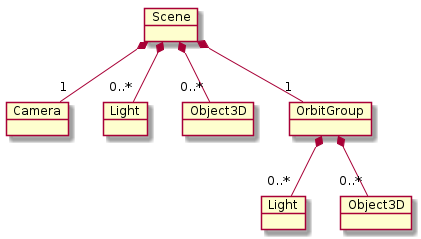
\includegraphics[height=5.5cm]{diagrams/out/c3_scene_graph.png}
    \caption{Ogólny graf sceny wizualizacji}
    \label{fig:c3_scene_graph}
\end{figure}

\subsection{Orbita globalna}

Orbitę globalną definiują dwa wektory - $g_v$ i $g_{up}$ na rysunku \ref{fig:orbits}. Pierwszy rozciągnięty jest od środka sfery do punktu, wokół którego orbituje kamera. Drugi jest wektorem jednostkowym do niego prostopadłym określającym orientację sfery w osi pierwszego wektora. W późniejszym opisie działanie \textit{na orbicie}, na przykład obrót orbity, oznacza wykonanie tej samej transformacji na obu wektorach. W ten sposób oba wektory nigdy nie zmienią swojej wzajemnej orientacji.

Użytkownik za pomocą myszy lub klawiatury może obrócić sferę, a konkretnie grupę obrotu (\texttt{OrbitGroup} na diagramie \ref{fig:c3_scene_graph}) i zawierane przez nie obiekty. Jest to efektywnie zmianą punktu, nad którym znajduje się kamera, pomimo tego, że jej pozycja się nie zmienia. Jako, że obrót sfery definiowany jest abstrakcję orbity, cała operacja sprowadza się do jej odpowiedniego obrócenia. 

Parametrami specyficznymi dla orbity globalnej są:
\begin{enumerate}
    \item tryb pracy orbity - określa czy podczas przesuwania orbity ma ona zachowywać swoją orientację w kierunku północnym. Wydzielono tryb \textit{swobodny} i \textit{kompas}.
\end{enumerate}

\subsection{Orbita lokalna}

Orbitę lokalną, podobnie jak globalną, definiują dwa wektory - $l_v$ i $l_{up}$ na rysunku \ref{fig:orbits}. Pierwszy rozciągnięty jest od punktu, wokół którego orbituje kamera, do kamery. Drugi jest wektorem jednostkowym do niego prostopadłym określającym orientację kamery w osi pierwszego wektora.

Użytkownik za pomocą myszy lub klawiatury może zmienić punkt orbitowania kamery. Jest to efektywnie zmianą położenia kamery w układzie obserwatora. Jako, że pozycja kamery definiowany jest przez abstrakcję orbity, cała operacja sprowadza się do jej odpowiedniego obrócenia.

Pierwszy wektor orbity lokalnej może mieć zmienną długość. Reprezentuje ona odległość obserwatora do punktu na powierzchni sfery. 

Parametrami specyficznymi dla orbity lokalnej są:
\begin{enumerate}
    \item współczynnik przybliżenia - jak powinna zmienić się odległość kamery od punktu na powierzchni sfery podczas jednej akcji przybliżenia.
    \item granice przybliżenia - minimalna i maksymalna odległość kamery od punktu na powierzchni sfery.
\end{enumerate}

\subsection{Parametry wspólne dla obu orbit}

Dla obu orbit wyróżniono wspólne parametry. Są nimi:
\begin{enumerate}
    \item granice - wyrażony w radianach zakres współrzędnych geograficznych definiujący fragment sfery, nad którym kamera może się znaleźć. Może służyć na przykład do ograniczenia obszaru poruszania się użytkownika tylko do jednej półkuli lub jednego miasta.
    \item prędkość obrotu - współczynnik sterujący prędkością obrotu danej orbity.
\end{enumerate}

Wszystkie parametry, ogólne i te specyficzne dla każdej z orbit mogą być konfigurowane przez wizualizację.

\begin{figure}[]
    \centering
    \newlength{\gRadius}
\setlength{\gRadius}{3cm}
\newlength{\lRadius}
\setlength{\lRadius}{4cm}
\tikzset{>={Latex[scale=1.5]}}

\begin{tikzpicture}[scale=1.25]
    \coordinate (G) at (90:\gRadius);
    \coordinate (G_up) at ($(G) +(0:1)$);
    \coordinate (L) at ($(G) +(135:2)$);
    \coordinate (L_up) at ($(L) +(45:1)$);
    \coordinate (center) at (90:0);


    \begin{scope}
      \clip (-\gRadius,0) rectangle (\gRadius,\gRadius);
      \draw[thick] circle (\gRadius);
  \end{scope}

    \draw[->] (center) -- (G) node[midway,left] {$\vec g_v$};
    \draw[->] (G) -- (G_up) node[midway,above] {$\vec g_{up}$};
    \draw[fill] (G) circle (1.5pt) node[above] {$c_g$};
   
    \draw[->] (G) -- (L) node[midway,above] {$\vec l_v$};
    \draw[->] (L) -- (L_up) node[midway,above] {$\vec l_{up}$};
    \draw[fill] (L) circle (1.5pt) node[above] {$c_l$};


\end{tikzpicture}


    \caption{Schemat orbit w specyficznym przypadku dwóch wymiarów}
    \label{fig:orbits}
\end{figure}



\subsection{Obrót orbity globalnej}

Algorytm obrotu orbity globalnej wykonywany jest dla każdego zdarzenia przesunięcia myszy użytkownika podczas gestu chwycenia, przeciągnięcia i upuszczenia wygenerowanym przez element \texttt{Canvas}. Obrót wymaga obliczenia jego chwilowej osi i kąta.

\subsubsection{Kwaterniony}
%TODO:Opisać

%TODO: wyliczanie osi i kąta obrotu + korekcja + korekcja trybu

\subsection{Obrót orbity lokalnej}

\subsection{Animacje - płynność ruchów}

\section{Implementacja}
